%%%%%%%%%%%%%%%%%%%%%%%%%%%%%%%%%%%%%%%%%%%%%%%%%%%%%%%%%%%%%%%%%%%%%%%%%%%%%%%%
%%% Methods
%%%%%%%%%%%%%%%%%%%%%%%%%%%%%%%%%%%%%%%%%%%%%%%%%%%%%%%%%%%%%%%%%%%%%%%%%%%%%%%%

\clearpage
\section{Methods and implementation}

To supply the required information and visualizations to the users I decided to use the process mining methods to analyze the event logs stored in the database.
I built my project into Jury, extending its functionality to provide detailed event analysis with visualizations.

I chose to use the theories from the \textalpha-algorithm to generate directed graphs describing the process model.
The graphs will be generated by analyzing several days worth of data from recent event log data. 
This way the graph dynamically adapts to change. 
Because of the several day long window the change is slow enough for the users to digest. 
However, I chose to generate the graphs based on user-supplied queries.
Hardcoded predefined values or graph shapes were to be avoided.
This way the time windows and event filters can be changed at any time without the need for a programmer to change the code.

The graphs were visualized to the users with two different views. 
The first view shows the directed graph to the user as is. 
The second view draws the graph on a timeline showing the activity start and end times.
The user can choose a previously generated model and overlay the real-time data on top of it.
Furthermore, the graph will include estimations for future events and their predicted times.

In this section I will go over the methods I used to solve the given problem in detail.
I will describe how they were implemented in the store systems.
I will also introduce the technology choices and explain how they were used to implement the methods.

\subsection{Chosen technologies}

The decision about which technologies I would use for my project was straightforward.
Since the project was to integrate with the existing Jury system, I chose to share its technologies and libraries.
Jury was built with C\#, running as an ASP.NET MVC application with .NET Framework.
The database was running on SQL Server, and the query engine was set up with an object-relational mapping tool called Entity Framework. 
\nyi{Need versions?} 
The approach used was a ``data first'' model \nyi{ref}, where the system automatically generates models (C\# classes) based on the database schema. 
\nyi{links, citations}
The user provided text queries were translated to database queries with LINQ. \nyi{elaborate?}
I used these same technologies in my project.

\subsection{Graph construction}

\subsubsection{Pre-processing}

To comply with the user requirements of being able to generate models from custom queries and real-time production data, 
the system developed in this thesis should be able to take any set of events as the input.
As outlined before, the system should use the textual query system to retrieve the events from the database.
The system will not have any knowledge of what filtering has been used, it only executes the user-given query.
The only check the system needs to do is to check the events against the current user's permissions, to protect confidential information.

The Jury system already had functionality to retrieve the events from the database based on a \emph{query}.
A query is a character sequence (a string) containing user-provided criteria for which events to show, based on the fields of the event entry (see table \ref{tab:event}).
For example, the user could be querying for a specific product or a specific submission ID.
A query ``\texttt{submissionid is 100100}'' would return all events from the specified submission.
Boolean operators familiar from search engines such as ``\texttt{and}'', ``\texttt{not}'', and ``\texttt{or}'' can be used to combine multiple conditions to form a more complex query.

After the query has been executed by Jury, the result is a set of events.
Jury displayed the set to the user as a plain timestamp-ordered list of events as seen in figure \ref{fig:plaineventlog}.
Because of the challenges outlined in section \ref{sec:datachallenges} a pre-processing step is necessary.
The plain set of events needs to be filtered and grouped into valid traces.

The pre-processing step takes a set of events as the input and works as follows:
\begin{enumerate}
    \item Drop events based on the user's permission level.
    \item Group all events by \textbf{submission ID}.
    \item Create a trace corresponding to a submission for each of these groups.
    \item Order all events in each trace by ascending timestamp, then by event ID.
    \item Drop all traces containing an event describing an error such as ones with a status ``Failed''.
    \item Drop all non-final events from each trace.
\end{enumerate}
After these steps the result is a set of \textit{valid traces} with only final events, each corresponding to a \textit{unique submission ID}.

By using different time slices or different filters on which events to include, we can generate models for different purposes. 
For example, we can try to generate a more accurate process model by filtering the events.
If we filter the events in the pre-processing step to only include events related to certain products
or product types, we can assume that the process model and the statistics will better describe those products.

However, filtering reduces the number of events used for the model, which can lead to overfitting.
For example, if the model is generated for only submissions that contain large file sizes, it may affect the results of the process discovery. 
In theory, some of the activity lengths could depend on the file size, meaning a query only containing large files may result in these activities always appear to complete later in the log.
This would result in inaccurate process models.
Because of this, care should be taken when creating models from small datasets.

\begin{figure}[htb]
    \centering 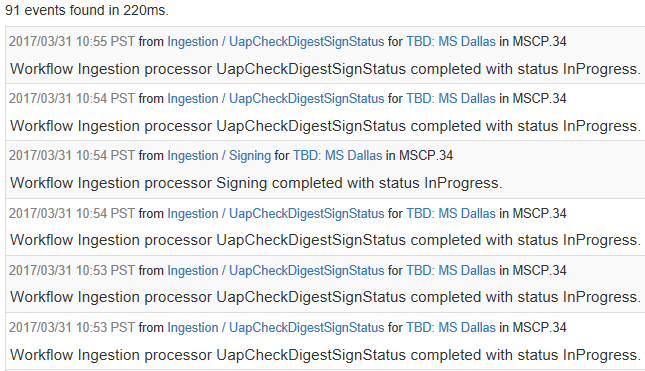
\includegraphics[width=0.7\linewidth]{gfx/screenshots/plaineventlog.png}
    \caption{Event log query result view in Jury}
    \label{fig:plaineventlog}
\end{figure}

I use the existing queries in Jury in my implementation to retrieve events from the database. 
The queries can be written by users and saved in the system.
These saved queries are then used to discover the process models.
Each model has a corresponding saved query.
For example, if the query searches for events belonging to only game products, 
then the discovered process model should reflect the underlying process specifically for games.
This allows for a highly flexible system where the users can create models for any subset of products or events that are relevant to them. 

\subsubsection{Creating directed graphs}

The model chosen to represent the process models is the directed graph. 
In this model, every pair of directly subsequent events $(a,b)$ appearing in a trace corresponds to a 
graph edge from node $a$ to node $b$.
The directed graph was chosen because of its familiarity to non-technical users since it resembles a traditional flowchart.
The parallelism is generated by observing the direct follow-relations similarly to the \textalpha-algorithm described in section \ref{sec:alphaalgorithm}.

To generate a graph from a set of traces, I started by generating an event log \emph{footprint matrix}.
The footprint matrix describes the relation of all the events in the log regarding to each other.
This means that the matrix describes which events immediately follow other events in the set of traces.
The columns and rows of the matrix correspond to all the distinct events (the event vocabulary).
The matrix is square and should have a zero diagonal, since each final event should only appear once in a trace.
The row describes the first event, and the column the event directly following.
The number in the matrix cell describes the frequency that this follow relation was observed in the logs.
This matrix is labeled the \textit{follow-frequency matrix}.
It can be generated by linearly traversing each trace once, and for each pair of subsequent events incrementing the number in the corresponding cell.

I will illustrate this with an example. Consider an event log with four activities $a,b,c,d,$ and $e$.
Figure \ref{fig:exampletraces} illustrates the six traces in the event log. There are two unique kinds of traces, $abcde$ and $acbde$, both of which have been observed three times. Figure \ref{fig:examplematrix} shows the footprint matrix generated from these traces.
The diagonal is zeroes, since no event follows itself.
Looking at the upper triangle the matrix we can see that $b$ has followed $a$ three times and $c$ has followed $b$ three times. From the lower triangle we see for example that $a$ has never followed $b$, but $b$ has followed $c$ three times.
By comparing the frequencies in the upper triangle to the lower triangle we can discover dependencies suggested by the event log, and from a lack of dependency we can suggest parallelism.

\begin{figure}
    \centering
    % example traces
    \begin{subfigure}[h]{0.4\linewidth}
        \begin{center}
        \begin{tabular}{| r | l |}
        Trace & Frequency \\
        \hline
        a b c d e & 3\\
        a c b d e & 3 \\
        \hline
        \end{tabular}
        \end{center}
        \caption{A list of example traces}
        \label{fig:exampletraces}
    \end{subfigure}
    % footprint example
    \begin{subfigure}[h]{0.4\linewidth}
        \begin{center}
        \begin{blockarray}{cccccc}
          & a & b & c & d & e\\
        \begin{block}{c(ccccc)}
        a & 0 & 3 & 3 & 0 & 0 \\
        b & 0 & 0 & 3 & 3 & 0 \\
        c & 0 & 3 & 0 & 3 & 0 \\
        d & 0 & 0 & 0 & 0 & 6 \\
        e & 0 & 0 & 0 & 0 & 0 \\
        \end{block}
        \end{blockarray}
        \end{center}
        \caption{An example footprint (follow-frequency) matrix $M$ }
        \label{fig:examplematrix}
    \end{subfigure}
    \caption{Example for traces containing events $\{a,b,c,d,e\}$}
\end{figure}

% turning the matrix into a graph
The generated footprint matrix corresponds directly to the event log based ordering relations described by van der Aalst and van Dongen \cite{van2013discovering,van2016process}.
There are four possible relations between any two events in an event log $L$:
\begin{itemize}
    \item $a \rightarrow_L b$: $b$ \emph{directly follows} $a$.
    \item $a \leftarrow_L b$: $b$ \emph{directly precedes} $a$.
    \item $a ||_L b$: $a$ and $b$ are \emph{parallel}.
    \item $a \#_L b$: $a$ and $b$ are not directly related, they are $unrelated$.
\end{itemize}

Note that $a \rightarrow_L b \Leftrightarrow b \leftarrow_L a$ is always true.
We can find these relations from the footprint matrix $M$ by comparing each cell $m_{ij}$ the upper triangle with the corresponding cell $m_{ji}$ lower triangle by using the algorithm described in definition \ref{def:logrelations}.

\begin{definition}
Let $A = \{ a_i | 0 < i \le n \}$ be a set of $n$ activities (the \emph{vocabulary}).
Let $M$ be an $n \times n$ footprint matrix corresponding to $A$.
For each cell $m_{ij} \in M$ where $i < j$:
\begin{itemize}
    \item $a \#_L b$ iff $m_{ij} = 0$ and $m_{ji} = 0$
    \item $a_i \rightarrow_L a_j$ iff $m_{ij} > m_{ji}$ and $m_{ji} = 0$
    \item $a_i \leftarrow_L a_j$ iff $m_{ij} < m_{ji}$ and $m_{ij} = 0$
    \item $a_i ||_L a_j$ iff $m_{ij} > 0$ and $m_{ji} > 0$
\end{itemize}
Furthermore, it should be noted that these relations are symmetrical:
\begin{itemize}
    \item $a \#_L b \Leftrightarrow b \#_L a$ 
    \item $a_i \rightarrow_L a_j \Leftrightarrow a_j \leftarrow_L a_i$
    \item $a_i ||_L a_j \Leftrightarrow a_j ||_L a_i$ 
\end{itemize}
\label{def:logrelations}
\end{definition}

In the example described before, comparing the cell $M[a,b] = 3$ to cell $M[b,a] = 0$ results in $a \rightarrow b$.
However, by comparing $M[b,c] = 3$ to $M[c,b] = 3$ the algorithm results in $b || c$. 
Figure \ref{tab:examplefootprint} shows the generated footprint for the matrix shown in figure \ref{fig:examplematrix}.
Note that it is enough to only examine the upper triangle of the matrix, since the generated footprint is always symmetrical across the diagonal.
If the rows and columns are ordered by dependency, the dependencies follow the diagonal of the footprint.
The parallel activities can be seen visually as square-shaped symmetric regions.
The parallel region border consists of follow-relations while the inside of the region contains parallel-relations.
This shape can be seen in the example figure \ref{tab:examplefootprint}.

This footprint maps directly to a corresponding directed graph.
Every activity in the vocabulary corresponds to a graph node.
Every ``directly follows'' relation corresponds to a directed arc (edge) in the graph. A parallel relation corresponds to arcs in both directions.
Figure \ref{fig:examplegraph} shows the directed graph corresponding to the footprint from figure \ref{tab:examplefootprint}.

\begin{figure}
    \centering
    % footprint table example
    \begin{subfigure}[h]{0.4\linewidth}
        \begin{center}
        \begin{tabular}{cccccc}
        \hline
          & a & b & c & d & e\\
        \hline
        a & \# & $\rightarrow$ & $\rightarrow$ & \# & \# \\
        b & $\leftarrow$ & \# & || & $\rightarrow$ & \# \\
        c & $\leftarrow$ & || & \# & $\rightarrow$ & \# \\
        d & \# & $\leftarrow$ & $\leftarrow$ & \# & $\rightarrow$ \\
        e & \# & \# & \# & $\leftarrow$ & \# \\
        \hline
        \end{tabular}
        \end{center}
        \caption{Generated footprint of log relations}
        \label{tab:examplefootprint}
    \end{subfigure}
    % directed graph example
    \begin{subfigure}[h]{0.4\linewidth}
        \centering 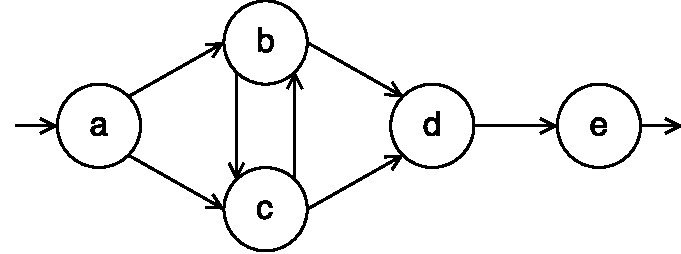
\includegraphics[width=\linewidth]{gfx/figures/graphthing.pdf}
        \caption{Generated graph}
        \label{fig:examplegraph}
    \end{subfigure}
    \caption{Graph generation from the footprint}
\end{figure}

% Dealing with noise
Noise in the event log data creates problems if it is not appropriately handled. 
Network delays, bugs, and other errors cause events to get lost or erroneously arranged in the traces. 
This noise manifests in the footprint follow-frequency matrix.

Figure \ref{fig:examplenoise} shows an example footprint matrix from a slice of production logs.
The frequencies shown in the figure are logarithmic for improved visibility.
As can be seen from the figure, two parallel regions of activities can be seen clearly in the data.
The first region contains three parallel activities, and the second one seven activities.
Within the regions, the frequencies observed are fairly constant.
However, outside the regions most cells still have non-zero values, even though the real process model
does not have parallelism between the leftmost and the rightmost activities.
This is the aforementioned log noise.
If left as is, the noise will create invalid arcs in the graph.

\begin{figure}[htb]
    \centering 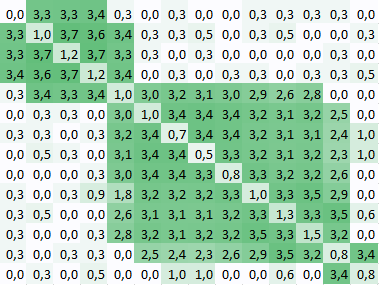
\includegraphics[width=0.6\linewidth]{gfx/graphs/noise.png}
    \caption{Observed noise in production data (logarithmic scale)}
    \label{fig:examplenoise}
\end{figure}

My method of dealing with the noise was to apply a threshold value to all the frequencies.
The value was a fraction $0 \le t_n < 1$ of the number of traces $N$ analyzed in the event log.
Any value in the matrix lower than $t_n N$ will be set to zero before the matrix is turned into a graph.
Similar thresholding will be performed when checking for parallelism (see definition \ref{def:logrelations}). 
For parallelism I calculate a fraction $d_p = \frac{f_\text{follow}}{f_\text{follow} + f_\text{precede}}$, where $f_\text{follow}$ is the frequency of follow relations from the upper triangle of the footprint matrix and $f_\text{precede}$ is the respective frequency from the lower triangle.
To counter noise, the relation is only considered to be parallel if the fraction is between the treshold values $t_p \le d_p \le (1 - t_p)$. 

Initial tests on the production data showed that relatively small ($t_n \le 0.01$) values were sufficient to counter the noise without affecting the model negatively. 
I used $t_n = 0.01$ and $t_p = 0.005$ to remove 1~\% of noise.

\nyi{Add figure for observed relations from excel}

% directed graph tldr
The result of this method is a directed graph with nodes and edges.
The graph describes the process model that was discovered from the event log.
Each node corresponds to an activity in the process model.
Each edge corresponds to a possible transition (pair of two consecutive events) in the trace.
The model can be verified by ``re-playing'' a trace as described in section \ref{sec:processmodelsdsc}.
Each event in the trace should correspond to a valid directed edge, with the first event of the trace being at the input node of the graph.

\subsubsection{Latency}
\label{sec:latency}

In addition to discovering the process model, one of the requirements was to see statistics of the times each of the activities take. 
Since the event timestamps describe the end time for each activity, the length (or duration) of an activity can be found by comparing the timestamps of two consequent events. 
I call this time difference between events the \emph{latency}.
The latency describes how much time is expected to pass until an event is followed by another event.
The latency can be seen as the length of an edge in the directed graph.

The statistics the users were interested in were the ``top percentiles'' (TP).
A top percentile is a value that corresponds to a set of numbers, such as all the observed durations of activities.
A $n$-top percentile means the value that is higher or equal than $n\%$ of all the values in such a set.
This can be expressed as the ``TPn'' value.
For example, the TP75 is the value that is higher or equal than 75~\% of all the values in the set.
TP50 corresponds to 50~\% and is equal to the median value of the set.
When looking at statistics about the store, the top percentiles have proven to be useful.
Looking at average values is often misleading, since the store systems often contain a very small amount of outliers with very high latencies, that skew the averages up.
The interesting statistics that were chosen are the TP50, TP75, and TP90. 
These correspond to the values used in other telemetry systems so they can be compared against for verification purposes.

In practice the TP values can be found by ordering the values in the set in an ascending order as an array, and then picking the index that corresponds to the percentile. For example, is the ordered array has the length of 1000 elements, the TP90 value can be found at the 900th index of the array.

My method was to collect the statistics at the same time as generating the graphs.
Since each cell in the footprint corresponds to an edge in the graph, I construct an array of latencies for each cell as I traverse through the traces.
When a number in the follow-frequency matrix is incremented, I also store the latency between the two events in the corresponding array. 
After the graph is generated, I can store the chosen key statistics (TP50, TP75, TP90) for each graph edge and discard the matrix and the arrays.

\subsubsection{Loading graphs from a file}
\label{sec:jsonfile}

As a secondary option, I developed a method to bypass the graph generation algorithm completely, and instead load the shape of the model from a JSON (JavaScript Object Notation) definition file.
By using a definition file, the engineers can ``force'' a template to have a specific exact shape.
This is useful in a few applications.
In some cases it is useful to have a ``stable'' graph with a pre-defined shape.
Since the algorithm is unsupervised and train itself constantly with a multiple day time window (e.g. the last 7 days), any changes made into the process may take the same time to become visible in the graph.
Additionally, small datasets can be too noisy for the algorithm to correctly identify the shape.
In such cases, the engineer can supply a JSON file.
This only affects the graph shape discovery. 
All the other parts of the systems work identically for both cases.
This feature can be toggled on a template by template basis, so both JSON-defined and automatically generated templates can be used side by side.

\subsubsection{Paging}
\label{sec:paging}

% implementation, paging
Many queries can return hundreds of thousands of events and visualizing all of them would be resource-intensive.
In addition, when discussing the requirements with the users they often only wanted to see the latest few submissions.
Because of these reasons I developed a paged view that visualizes the events retrieved from the user's query, but restricts the number of graphs shown to the user in a predictable way.

First, I run the user's query and retrieve the events, filtered by the user's permission level.
I sort these events by descending timestamp and pick the five latest submission IDs.
These IDs will correspond to the five latest submission traces matching the user's query.
``Latest'' in this context means the traces with the most recent activity.
Optionally, the user may select to see the traces ordered by the latest start time.
This query may also be paged, allowing the user to choose the next five traces, or any later set of five.
After five submission IDs has been retrieved, they are used to query all events belonging to these submissions. This results in five traces that can now be processed.

This is implemented with two SQL queries.
The first query that retrieves the five submissions can be paged with a standard page selector user interface component.
This means that the user can choose to see the next ``page'' of submissions containing submissions 6-10 and onwards.
The first query uses a \texttt{GROUP BY} clause to group the events by submission ID and to choose the maximum timestamp.
This result is then sorted and the top five IDs are selected.
This selection can be paged with a SQL \texttt{OFFSET} clause based on the user's page selection.
The query runs in only a couple seconds on a cloud-hosted SQL Server instance.
The second query retrieves all events that belong to the retrieved five submissions.
These events are then passed to the graph generation algorithm.

\subsubsection{Storing the graphs}
\label{storinggraphs}

As described before, the project allows the users to generate new graphs from any query supplied by the user.
Reading hundreds of thousands of events from the database, sorting them and generating the graph takes a lot of time, in the order of several minutes.
Creating new graphs from a previously unseen query is resource-intensive, so the functionality is restricted to the system administrators in Jury. 
Since Jury is an online tool the service response times need to be fast, preferably in the order of a fraction of a second, to preserve a smooth user experience \nyi{cite?}.
Generating the graph from a set of events for each web request from any user would be inefficient and the page load times would be in the order of minutes.
Because of this, I implemented two levels of caching in the system.

The Jury web server is distributed onto multiple server instances to provide high availability. The database server is shared between the instances.
Each generated graph is cached both in the database and locally in memory at a server instance.
The in-memory cache is local to each instance and the database cache is shared.

Each cached graph is associated with a timestamp corresponding to the time when it was generated. 
This timestamp is used by the servers to determine when the cache is too old and should be refreshed.
For the in-memory cache this maximum age was chosen to be 15 minutes.
For the database cache the maximum age was set to 12 hours.
The long time was chosen to be sufficient for the store backend system.
While the process model of the store system changes constantly when improvements are made, the changes happen over several days rather than hours. A day old cached model will be accurate in most cases.

The cache system works as follows (from the perspective of a single server instance):
\begin{enumerate}
    \item The server receives a HTTP request requiring a specific graph.
    \item The server reads the timestamp (age) of the in-memory cache. \\
    \textbf{Graph not in memory}: Continue to the next step.
    \textbf{Less than 15 minutes old}: Return the graph from memory to the user and stop. \\
    \textbf{Older than 15 minutes}: Return the graph from memory to the user and continue to the next step in the background.\\
    \item The server reads the timestamp (age) from the graph stored in the database.\\
    \textbf{Less than 12 hours old}: Load graph from the database, store it in memory. Return to user if needed.\\
    \textbf{Older than 12 hours or not in database}: Move the graph timestamp in the database 15 minutes forward and generate a new graph. Once the task is finished, save it in the database, and in memory.
\end{enumerate}

If the requested graph is in memory, it will be returned to the user immediately. 
If the version in memory is too old, a background task to retrieve or generate a new graph is started. 
The graph in memory is returned to the user regardless. 
This means that the user almost never has to wait for the page to load while the graph is being generated.
The only case when the user has to wait for the graph generation is if the instance has no graph in memory and the version in the database is also too old.
In practice this will only happen after a server restart when all the in-memory caches are purged.

The graph timestamp is moved 15 minutes forward at the start of graph generation to prevent a situation where two different server instances are generating the same graph separately.

This two-level caching improved the page loads from minutes to fractions of a second. Furthermore, since the graphs are now stored also in the same database as the events, they can be used in SQL queries. This proved to be useful, since SQL queries can be constructed to improve the notification functionality. See section \ref{sec:notifications} for more details about notifications.

\subsection{Real-time functionality}

Until this point I have considered the case of the event log that corresponds to a time slice of past data.
This type of data can be seen as an ``aggregate'', since it will result in a model that describes events over a long period of time.
However, a key part of the analytics for the store is the ability to analyze and debug the current state of the system.
Without such functionality it will be difficult to analyze the state of the current submissions in the system.

As outlined before, the system already had a view to list events based on the user's query, as seen in figure \ref{fig:plaineventlog}.
I call this the \textbf{log view}.
The users of the system reported that this view was useful for debugging a specific issue for e.g. with a specific activity, but it does not provide a good overall view.
The request from the users was a view that would show a big picture of the status of a submission with the option to drill down to the details.

% new small dataset from a query, often a single trace
My solution was to leverage the previously discovered aggregate model for visualization.
The model would be combined with the list of events returned by the query.
The aggregate model would be used to visualize the process, and the real-time data from the query would be ``overlayed'' on top of the model.
In other words, the idea was to ``color'' the model with the real-time data from the query.

The query returns a set of events that corresponds to the user's criteria.
For simplicity we can assume that the result is a single trace for an ongoing submission,
a set of sequential events that all belong to a single case.
In the final implementation the result can also be events from many separate submissions.
The system handles it by splitting them into separate visualizations and then handling each one of them as a separate case.

In the beginning we create an ``colorless'' graph by copying the process model discovered earlier.
The colorless graph has a node for each activity and the corresponding graph edges between them.
The nodes are tied to the specific activities by including the Source and Subsource fields. 
These colorless nodes have no status, timestamp, or other metadata.
The visualization is ``colored'' by traversing through the trace in sorted order (ascending timestamp).
For each event in the trace, I find the corresponding node in the graph.
It is then ``colored'' by copying the status, timestamp, and other metadata from the event to the node.
This can be repeated until we reach the end of the trace.
The result is a ``colored'' graph where all the activities that have been finished have a status and a time.
The nodes for the activities yet to come remain uncolored.

\nyi{Does this need an illustration?}

This graph can now be shown to the user.
The nodes are drawn on the screen as circles or rectangles, and the directed edges as arrows between them.
This is what I call the \textbf{graph view}.
The parallel nodes are connected by double-sided arrows or an edge that otherwise indicates the parallelism.
In my visualization I took the ``colorization'' quite literally by having each status correspond to a real color shown to the user.
Uncolored nodes remained grey, completed nodes green or blue, nodes in progress yellow, and failed nodes red.
The colors help the user to get an immediate understanding of what the state of a submission is.
An example of a colored graph can be seen in figure \ref{fig:coloredgraph}.

\begin{figure}[htb]
    \centering 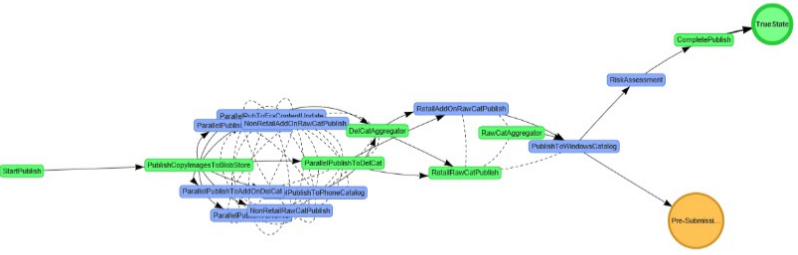
\includegraphics[width=0.9\linewidth]{gfx/screenshots/graphcolor.png}
    \caption{Colored graph view}
    \label{fig:coloredgraph}
\end{figure}

In my implementation I had to add one hard-coded aspect to cover an edge case. 
In the store system, it is possible for a publisher or a developer to ``re-publish'' a product. 
When a re-publish is triggered, the publishing steps of the workflow are run again with the same submission ID. 
This means that a trace from a single submission may contain several publishes.
My implementation detects when the first step of the publishing workflow is seen a second time in a single trace. 
When this happens, the trace is split into two and the re-publish will be shown as a separate trace in a separate visualization.

\subsection{Estimating the future}

One of the requirements discovered (see table \ref{tab:userneeds}) was to be able to provide estimations for the submission workflow completion times (labelled \emph{estimated time of arrival} or ETA). 
To provide such estimates I developed a method to traverse the graph forward after it has been colored.

% Estimating future on incomplete logs
The algorithm used in the project was a recursive traversal by using a stack.
The input for the algorithm is a graph which has been partly colored by a trace.
This means that some of the graph nodes have timestamps and metadata, while others (towards the end of the workflow) do not.
The goal is to use the previously generated process model to estimate
and fill in the data for the uncolored nodes.

% Statistical approach by using TP75
To fill in the data for future nodes, the algorithm needs a measure to be used for the estimation. 
This measure corresponds to the estimated ``edge length'' for each edge in the graph.
A simple approach is to use the statistical values that were collected during the graph generation process (see section \ref{sec:latency}).
The statistics are useful since the users prefer a ``worst case'' estimation rather than a ``best case'' one.
If a workflow finishes earlier than estimated, it is seen as a positive surprise by users.
For example, using the TP90 value should lead to an estimation that estimates the latencies in a way that overestimates 90~\% of the submissions.
However, choosing the right statistic is challenging.
The choice is a trade-off between avoiding underestimation and making an accurate prediction.
The plan was to use machine learning to improve the estimations (see section \ref{sec:ml-estimation}).

\nyi{pseudocode?}

\subsubsection{Estimation algorithm}
% algorithm description
First the algorithm finds the node which has the earliest timestamp.
This is treated as the graph start.
An empty stack is initialized and the start node is pushed into the stack.
After this initialization a recursive step is executed in a loop until the stack is empty.
In theory, since all the graphs are workflow graphs no loops should appear in the graphs (see ``connectedness'' in section \ref{sec:processmodelsdsc}). 
In practice, aspects like noise, errors, and changes in the system can lead to invalid graphs containing loops.
An empty list is initialized to keep track which nodes of the graph have already been visited.
The purpose of the list is to prevent a loop in the graph causing infinite execution or a stack overflow.

The recursive step starts by popping a node (called the \emph{current node}) from the stack and checking if the node is valid.
Validity means checking that the node has not been visited already, that the node is not an error state, and that the node has a timestamp.
If the node has been visited already it is ignored.
Error states are seen as anomalous and since they often lead to the workflow being aborted they should not be used for estimations.
The node needs to have a timestamp, otherwise there is no reference point for calculating an estimation.
After the node has been deemed valid, it is marked as visited.

After the initial check all children for the node are retrieved.
This means finding all the edges that have the current node as the source, and collecting the nodes that the edges point towards.
For each of these nodes, the estimation is performed.
If the child node already has a timestamp from the coloration phase, it is ignored.
Otherwise, if the node is uncolored, the previously chosen edge length measure (such as the TP75) is used for the estimation. 
The length of an edge is a length of time (a time span), corresponding to an estimate for how much time will pass between the two events.
By adding the time span to the timestamp of the current node, we get the estimation for the timestamp of the child node.

For parallel nodes (the nodes with a directed edge both to and from the current node) the step differs slightly. 
Since the activity corresponding to the node is known to be parallel to the current one, the edge length is seen as zero.
For this reason, the estimation step does not add anything to the timestamp but instead just copies the current node's timestamp to the parallel node.

After the timestamps of the child nodes have been estimated the child nodes are added to the stack and the step is performed again.
This continues until the stack is empty.
The stack will be empty when all the nodes connected to the starting node have been visited.
This means that, barring error states, every node will now either be colored or have a timestamp estimation.
These estimations can be shown to the user when the graph is visualized.

\subsubsection{Timeline view}

During the protyping phase I discovered that the directed graphs were not intuitive to read for the users.
Trying to manipulate the graph shape and selecting each node to see the details turned out to be cumbersome to the users.
Two users wished for a ``sorted'' view in the initial tests.
The sorted view should show the events arranged by time horizontally across the screen.
This resulted in the second prototype which I labelled the \textbf{timeline view}.
A basic example of what a timeline is can be seen in figure \ref{fig:basictimeline}.
The timeline has items set on a horizontal axis.
The horizontal axis corresponds to time, with past being on the left and the future on the right.
The vertical axis has no meaning other than to separate the parallel items visually to help the user see which activities happen in parallel.

\begin{figure}[htb]
    \centering 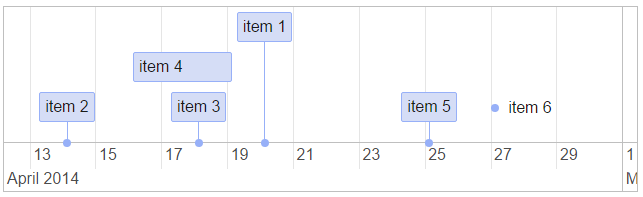
\includegraphics[width=0.6\linewidth]{gfx/screenshots/basictimeline.png}
    \caption{A basic example of a ``timeline'' \nyi{make a better one}}
    \label{fig:basictimeline}
\end{figure}

% Generating a timeline view with start and end times from the overlay
As can be seen from figure \ref{fig:basictimeline}, each item in the timeline has a width.
This means that the items have a both a \textit{starting time} and an \textit{ending time}.
However, in the event log each event only has a single timestamp corresponding to the ending time of an activity.
Since the event logs do not have any information about the starting times, the only option is to make an estimation.
To find the estimated starting times, I leveraged the process model graph again.

% Methods of finding the start times and dealing with parallelism
In my project I made the assumption that switching tasks takes a negligible (zero-length) time.
This means that when a task ends, the next task begins immediately.
With this assumption I can discover the starting time by looking at the end time of a previous task.
I can find the previous task by following the graph edges backwards and finding its dependencies.
The estimated starting time of the activity is the latest ending time of these dependencies.
In this method, all parallel tasks are treated equal, so each activity also must take into account all dependencies of its parallel tasks.
In the case where there are no dependencies (such as the first activity of the graph) a predetermined length will be used as a fallback.

In other words, before estimating the start times the timeline has all events as zero-width having only the activity end times. The algorithm sets the start time to be the earliest possible time without breaking the restrictions given by the process model dependencies.
After this step, all items in the timeline correspond to an activity and have a start time and an end time.
When the timeline is visualized the items can be separated by color (or other means) to distinguish between real-time information and estimations.
Furthermore, since the horizontal axis corresponds to time, the current time of the user can be shown as a vertical line.
This helps to highlight the current time to the user and to separate future estimations from observed events.

\nyi{add picture of a finished timeline}

\subsection{Machine learning}
\label{sec:ml-estimation}

% How ML approach could be used to improve the statistical approach
After I had implemented the statistical estimation, the next step was to research whether it could be improved by using machine learning. 
The idea was that for each graph edge, instead of using a statistical value to estimate the length, a machine learning model could be used.
The model could take into account the current time and transition, in addition to other characteristics of the submission such as details about the application package.
The hypothesis was that characteristics such as the package size have a predictable effect on the latencies.
To test this hypothesis I collected a set of training data from the production environment and used it to train and test machine learning models.
Had the model accuracy been proven to be more accurate than the statistics, the model could have been deployed to the production system.

% Explain models used (poisson \cite{azurepoisson}, bdt \cite{azurebdt} \cite{lambdamart2010})
% data suitability
% result interpretation
The machine learning models used in training were Poisson Regression \cite{azurepoisson} and Boosted Decision Trees \cite{azurebdt}.
These two were used as alternatives and they were compared against each other.
The better performing model was to be used in the final product.
These two models were chosen for testing based on a few factors.
The first factor was that the model needs to suit the data.
Since the latencies are based on the probability of an event happening, they fall on a Poisson distribution. 
This is why a Poisson Regression model was selected.
The Boosted Decision Trees model had been used before in the store for application classification with good results, so it was believed to work well with the feature set that I had available for the applications.

Second factor for choosing the models was the ability to interpret the results.
Since this project was experimental and there was no baseline, I wanted to be able to inspect the models and reason about their characteristics.
Since both the Poisson Regression model and the Boosted Decision Trees output the per-feature weights for the model, they can be inspected and reasoned about.
Compared to something like a neural network, which is highly challenging for humans to interpret \nyi{citation needed} this is a clear advantage.
The best model based on prediction accuracy was to be chosen for an in-production test.

% accuracy
% training / regression speed
Mean absolute error and the mean square error values were to be used to evaluate model accuracy.
Lastly, if multiple accurate models was to be found, the model training and regression performance would be used to evaluate them.

\subsection{Feature set}
\label{sec:featureset}

% Explain training dataset generation
The training dataset was generated from a time slice of the event logs. 
By using both a predetermined process model by using a JSON file (see section \ref{sec:jsonfile}) and the automatically discovered process model, two datasets were created. 
The datasets will be referred to as the ``JSON template'' dataset and the ``Automatically generated template'' from now on.
The datasets contain the observed values for the latencies, labelled by the activity transition and the application it belongs to.
These rows were then joined with a dataset of known applications and their characteristics to create the final training data.
The resulting dataset consisted of 16 columns of features such as the package size and the current transition (activity being observed), and a label column corresponding to the measured latency in seconds. 
See table \nyi{ref} for an example.
The data was filtered to only contain measurements from valid traces with the requirement of having no errors and conforming to the process model.
The datasets and their headers were anonymized before they were used to train the models.
Any information identifying a specific product was removed.
Furthermore, the column headers were replaces with generic ones, since the name of a column does not affect the result of the training.
The datasets used contain 36~982 rows for the JSON generated template, and 18~860 rows for the automatically discovered template.
The data reflect three days of event log data.

\nyi{Add table with example rows}

% Explain initial testing
% Testing with noisy features removed (textual fields)
The features used in the data were chosen based on experimental testing and domain knowledge.
Initially, data included fields such as the application description, keywords, and other developer-supplied textual information. 
However, these were deemed noisy and they drastically increased the training time because they required n-gram generation.
The domain experts (the system engineers) knew to inform that those fields are not used in the ingestion pipeline so they were removed from the datasets.
After the removal 12 features read from the application package characteristics where used. 
The data included numeric features such as the package size in bytes and some count data from the store related to how many previous submissions the application has.
There were also binary (true or false) features describing characteristics of the package, such as what kind of hardware permissions the application needs to have.
The two features read from the event logs were the current time in seconds since the submission start, and an enumerator for the current transition (the activity in question).
The label column was the latency (the duration of the activity) measured from the event log.

% Explain additional features
% identical resubmission
After the initial testing, two additional features were added to the dataset.
The first additional feature was a boolean value describing whether the application package is identical to the previous submission.
This was because the domain experts knew that this would lead to some of the activities skipping execution internally, drastically reducing the execution time for a couple specific activities. 
This was also clearly seen in the data when the latency distribution for an activity were plotted. 
Figure \ref{fig:resubmissions} shows that there is a clear divide between two sets of latencies.
The lower set of latencies are caused by the system detecting an identical submission and skipping the activity.
With this graph the training data could be split into two sets labelled by whether the submission is an identical resubmission.
%  posting that needed human interventiondcxfkkkkkkkkkkkkkkkkkkm
%                                       a cat did this ^ 
The second additional feature was whether the application ingestion triggered a manual review (human curation). 
Since orchestrating human manual reviewers contains overhead, a manual review is known to delay the ingestion time considerably.
This can seen from a latency distribution graph as a clear difference for the steps related to curation. 
Figure \ref{fig:manualreview} shows this effect in the distribution of the curation latency.
This knowledge was used to add the manual review boolean feature into the dataset.
I performed more tests with these two additional features to test whether they improved model accuracy.

The best performing models within a model class (such as the BDT) were found by running multiple models with different parameters in parallel and choosing the model with the best performance.
Initially the models had random (or default) parameters.
After the parallel tests the best performing model was selected as the baseline for the next iteration and the next set of models.
The iteration was repeated until better performed models could not be found anymore.
The resulting parameters and their error values from the tests can be found in section \ref{sec:results}.

\begin{figure}[htbp]
    \centering 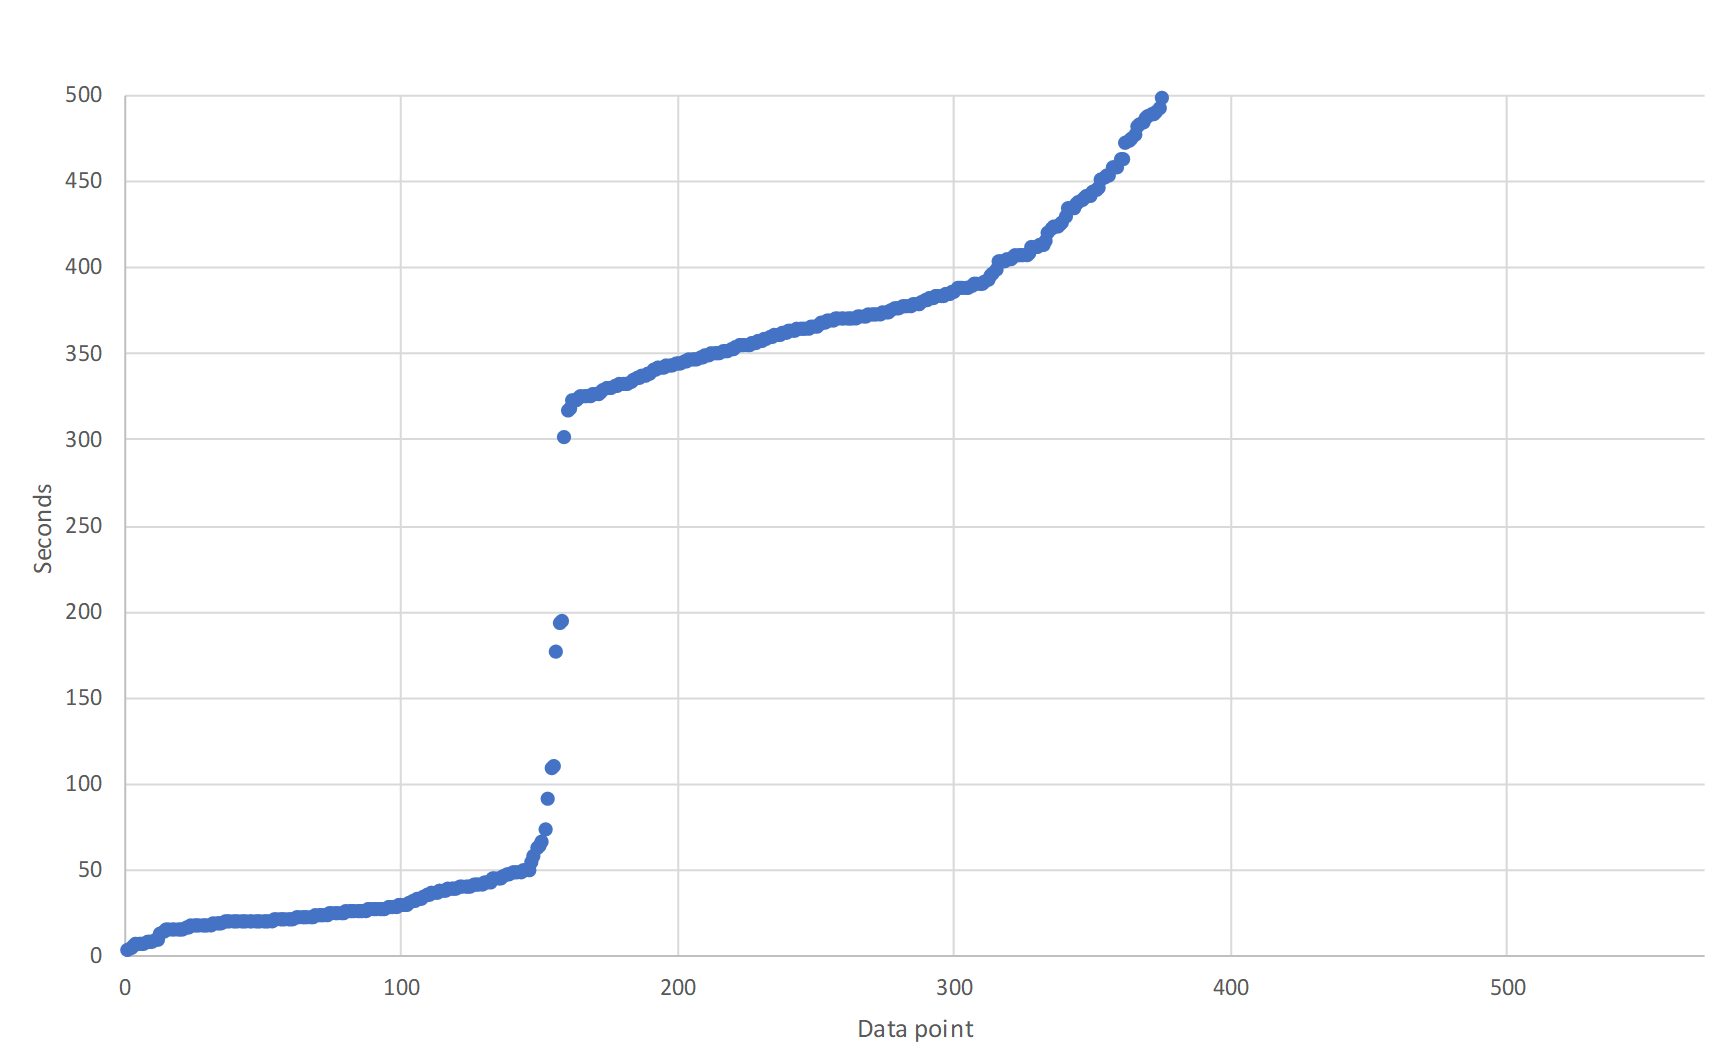
\includegraphics[width=0.9\linewidth]{gfx/graphs/resubmissions.png}
    \caption{Latency distribution divide caused by re-submissions}
    \label{fig:resubmissions}
\end{figure}

\begin{figure}[htbp]
    \centering 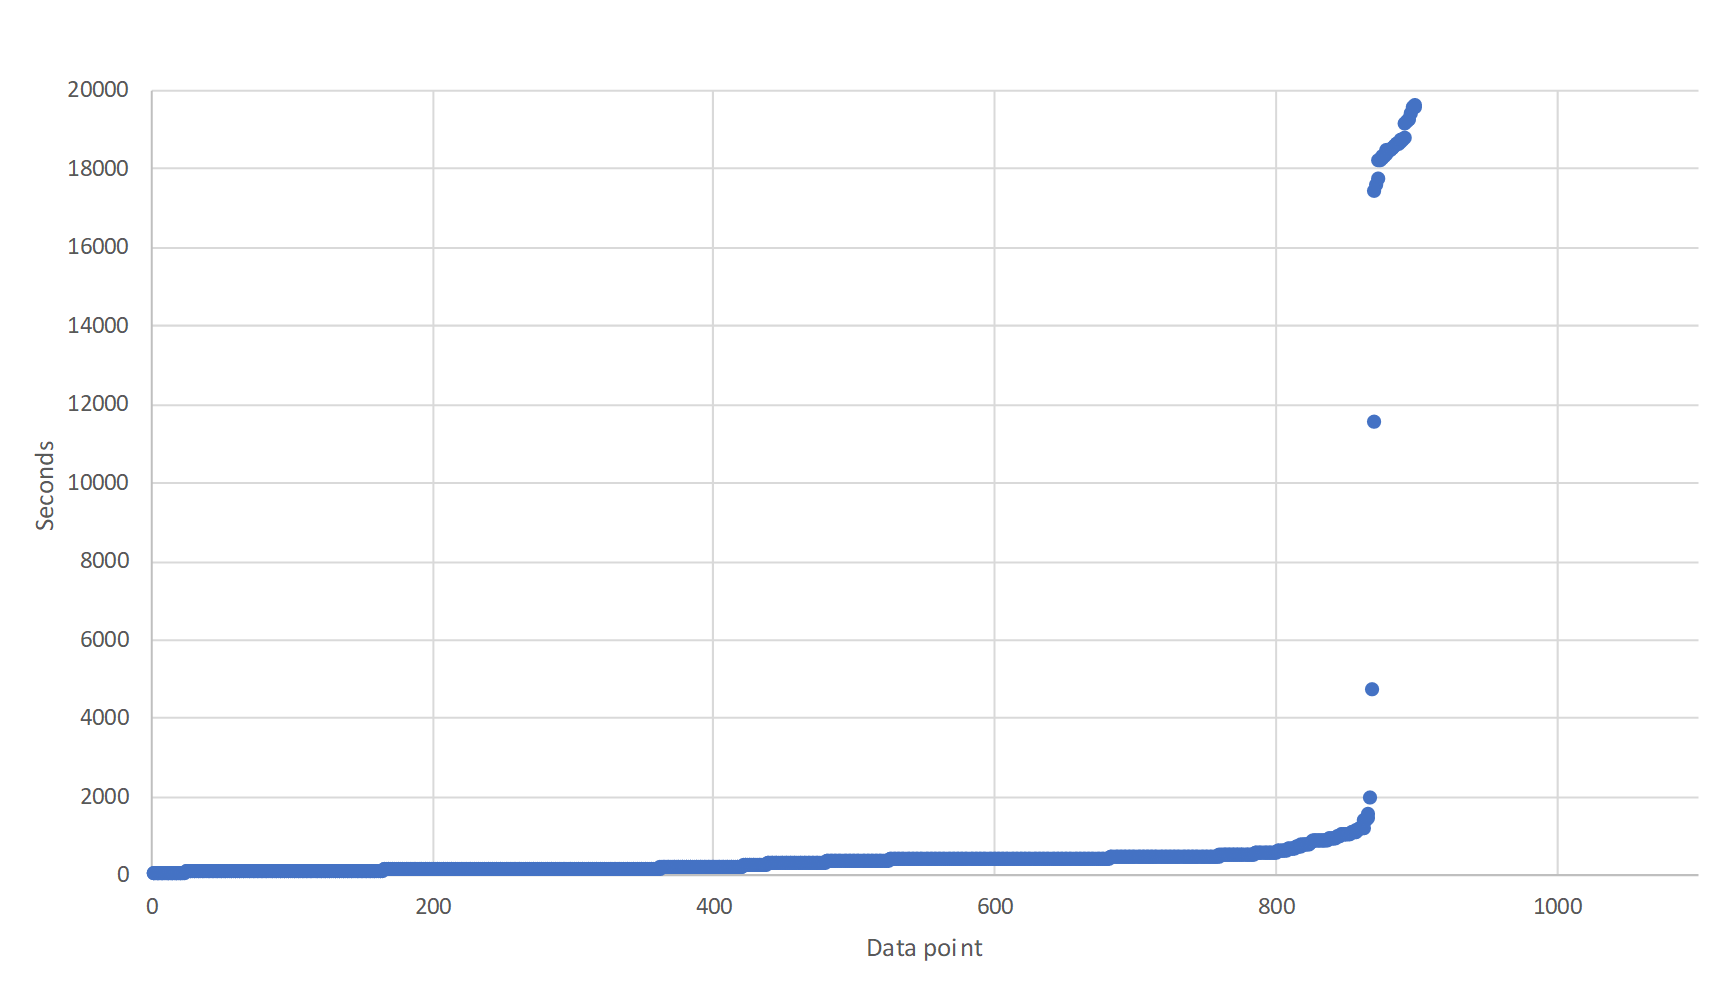
\includegraphics[width=0.9\linewidth]{gfx/graphs/manualreview.png}
    \caption{Latency distribution divide caused by entering manual review}
    \label{fig:manualreview}
\end{figure}

\subsection{Notifications}
\label{sec:notifications}

One of the main features of Jury is the ability for the user to request notifications for any events that are relevant to them.
The users can run queries and ``subscribe'' to them.
Whenever an event arrives to Jury which matches a subscribed query, a notification such as an email is sent to the user.
This allows Jury to notify the user for example when a product they are interested in receives an update or when an error happens.
Because the notifications use the same queries as the other parts of Jury, they allow the same high level of customization.

However, notifications were only triggered as a response to an incoming event.
This means that if an event was missing or delayed no notification could be sent.
Similarly, no notification could be sent about a workflow activity when it started, only when it was completed.

Receiving notifications for delayed submissions was a requirement discovered from users (see table \ref{tab:userneeds}).
Furthermore, notifying about a workflow activity before it happens was seen to be useful for scheduling purposes.
This functionality, or the data required for these functions, was not available in the old Jury system.
However, after I cached the process models and their statistics in the database (as described in section \ref{storinggraphs}) this data was now available in the same database as the events.
This allowed for SQL queries to be created to detect when an event is ``late'' before it even arrives.

For detecting late events, the system needs to examine the current ongoing submissions and the events that have been received already.
The submissions and their latest events can be found with a \texttt{GROUP BY} query as described in section \ref{sec:paging}.
In addition, each transition (graph edge) in a process model is associated with its statistics. 
This means that when the edge is stored in the database it also contains numeric values for the statistics such as the TP50, TP75, and TP90 (see section \ref{sec:latency}).
The latest event and the process model can be used to find the next expected transition for each event.
I did this by joining the latest events with the process model graph edge that corresponds to that event.
By adding the time span from a chosen statistic (such as the TP75) to the timestamp of the event I form an ``estimated time of arrival'' (ETA) for the next expected event.
If the current system time is past this ETA, we know that the next event is currently ``late'' and should have already been received based on the statistic chosen.

% tolerance, absolute and statx2
Because of the natural randomness and varying small delays in the system, choosing a good statistic is crucial. 
For example, if I used the TP75 as the statistic for late event notifications, even in the ideal case the user would be notified 25~\% of the time.
Furthermore, the users generally are not interested in event being very slightly late (such as a couple minutes) but only after the event is ``considerably'' late.
What ``considerably late'' means should be chosen by the user, not the developer, since the user is the domain expert.
Similarly, some activities are very short in length so even a one minute delay caused by the clock skew can seem like a large relative delay.
In addition, some activites may involve absolute contractual SLA times that are critical and should not be based on statistics but rather an absolute value defined by the contract.
The user is the expert knowing the activities and their characteristics.
For this purpose the choice of what is considered ``late'' is left to the user.

After my process models were available in Jury, a colleague implemented the ``lateness'' syntax into the Jury query language. 
This allows the user to add a keyword \texttt{latest} to the query to run the previously described \texttt{GROUP BY MAX(timestamp)} query.
Tthe user can add filters for ``lateness'' such as to only show events that are delayed for more than two times the TP75 value.
The user can also supply an absolute value, or a combination of these two.
For example, the user may want to be notified for events that are later than two times the TP75 value, but only with a minimum value of five minutes of delay.
Because all this was added to the query language, no new notification system was needed since Jury could already notify based on queries.

\subsection{User interface}

The main purpose of this project was to help users understand the event data in Jury.
Visualizations played a key role in giving the users the ``big picture'' of the submissions and the real-time status of the products.
Since the users were mostly not developers, the visualizations needed to be easily accessible.
The visualizations should be intuitive and easily readable by possibly non-technical users.
This needed a graphical user interface integrated directly to Jury.

For the visualizations I used a JavaScript library called \emph{vis.js} \cite{visjs} that was already being used elsewhere in Jury.
The library supports drawing and manipulating graphs with nodes and edges in the client browser.
Furthermore, the library supports drawing activities on a timeline out of the box.

The events section of Jury was to have easy access to the three different views outlined before: the log view, the graph view, and the timeline view. Furthermore, the user should be able to select the process model that they want to use for the visualizations.
For example, an user examining a game submission may want to use the aggregated process model from several days of only game submissions.

As explained before, the process models can be generated from any user-supplied queries.
However, the team decided to not allow any user generate a model from any query, since processing hundreds of thousands of events to generate a new model is very resource-intensive.
Only users with admin privileges in Jury were to be able to save queries as new process models.
The admin user can then choose to publish the model to be used by everybody.
We chose to call these published models ``templates'', since they affect the visual shape of the graph in the visualizations and the word was easily understood by non-technical users.
The real-time data is then overlaid on the template.

I also implemented a fallback option for using templates not generated from log data. As described in section \ref{sec:jsonfile} the store engineers who have developer access to Jury can supply a JSON configuration file containing the shape of the process model. The format of the file was chosen to be the same than what was used in other store backend systems. 
When using the supplied template file, the system skips the step where past events are fed through the algorithm, and instead reads the shape of the model from the file.  
This enables the option of having a template in the system that never changes without developer action, for example for debugging purposes.

The user interface was designed with these three goals:
\begin{itemize}
    \item The user should be able to switch between the three views without losing prior input such as the search query.
    \item The user should be able to select the template from the admin-specified queries.
    \item The interface should help the user find the right keywords and drill down to specific submissions if multiple are shown.
\end{itemize}

To accomplish the goals the views were set up with a shared header and toolbars.
The main header with the search bar on top of the page remains the same across all the pages of Jury.
Furthermore, all the event pages share a secondary header that enables switching between the detailed log view and the visualizations. 
It allows the user to select the template (the process model) used for the visualizations, which will be shared between all the search results.
In addition, each visualization (both in graph view and timeline view) includes its own header showing the basic details about the submission, such as the product name and submission ID. The header also includes shortcuts specific to the submission shown, such as links to queries that only return events belonging to the same submission.
A small ``hamburger menu'' button on each submission includes links to other parts of Jury, such as links to the publisher information, the product information, and to other systems that may have related information.

Using vis.js for the visualizations was straightforward after my algorithms had already generated the graphs on the server side. 
On the client side (in the user's browser) I only needed to supply vis.js with a JavaScript object containing a list of nodes and a list of edges. When supplied with additional options about the desired layout, vis.js builds a graph and fits it in the view automatically. The user can even manipulate the graph with the mouse to rotate the graph. The graph has simple two dimensional physics where the edges act as springs.

However, the users did not like this visualization. The moving nodes and springs were seen as ``chaotic'' and ``annoying'' rather than useful. 
The users requested sorting or ordering functions for the view, such as aligning the nodes on a horizontal axis. 
This is why the timeline view was implemented. 
Similarly as the graph view, vis.js draws and arranges the timeline automatically when supplied a list of nodes with start and end times.
My algorithm already generated this information, so implementing it was only about formatting it to the right kind of JavaScript object.

The user interface was constructed in an iterative manner, rather than all at once. The link targets, positions, and sizes were adjusted based on what the users wanted. Most of this was done during the second half of my project.
After adjusting to the users' feedback, the user interface and the event system was released to production to Jury to be used by any Microsoft Store employee.

\nyi{Make sure the difficulties are all mentioned somewhere}\\
\nyi{(you'll want these for the presentation)}\\
\nyi{ - parallelism}\\
\nyi{ - clock skew}\\
\nyi{ - changes in workflow}\\
\nyi{ - bugs manifesting in graphs (is this really a bad thing?)}\\
\nyi{ - dealing with rare events (manual review)}\\
\nyi{ - confidentiality}\\
\nyi{user interface features discovered at mid point ??}